\section{Bonus: Style and Content Disentanglement in SVHN}

A curious property of the SSVAE graphical model is that, in addition to the latent variables $y$ learning to encode the content 
(i.e. label) of the image, the latent variables $\bz$ also learns to encode the \textit{style} of the image. We shall 
demonstrate this phenomenon on the SVHN dataset. To make the problem simpler, we will only consider the 
\textit{fully}-supervised scenario where $y$ is fully-observed. This yields the fully-supervised VAE, shown below in Figure \ref{fig:fsvae}.

\begin{figure}[h]
    \centering
    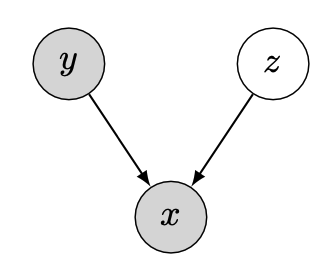
\includegraphics[width=0.15\textwidth]{./figures/fsvae}
    \caption{Graphical model for FSVAE. Gray nodes denote observed variables.}
    \label{fig:fsvae}
\end{figure}

\begin{enumerate}[label=(\alph*)]
    \item \input{05-fsvae/01-extracredit}

    \item \points{5b} Implement the \texttt{negative\_elbo\_bound} function in \texttt{fsvae.py}. In contrast to the MNIST dataset, 
    the SVHN dataset has a \textit{continuous} observation space

    \begin{equation} \label{eq:31}
        p(\bz) = \calN(\bz \mid 0, I)
    \end{equation}

    \begin{equation} \label{eq:32}
        p_{\theta}(\bx \mid y, \bz) = \calN\left(\bx \mid \mu_{\theta}\left(y,\bz\right), \text{diag}\left(\sigma_{\theta}^2\left(y, \bz\right)\right)\right)
    \end{equation}

    To simplify the problem more, we shall assume that the \textit{variance is fixed} at

    \begin{equation} \label{eq:33}
       \text{diag}\left(\sigma_{\theta}^2\left(y, \bz\right)\right) = \frac{1}{10}I
    \end{equation}

    and only train the decoder mean function $\mu_{\theta}$. Once you have implemented \texttt{negative\_elbo\_bound}, run
    \begin{verbatim}
        python main.py --model fsvae --train 
    \end{verbatim}

    To use GPU acceleration run the command below. 
    \begin{verbatim}
        python main.py --model fsvae --train --device gpu
    \end{verbatim}

    The default settings will use a max iteration of 1 million. We suggest checking the image quality of 
    $\text{clip}\left(\mu_{\theta}\left(\text{y,z}\right)\right)$—where $\text{clip}(\cdot)$ performs element-wise clipping of 
    outputs outside the range [0, 1]—every 10k iterations and stopping the training whenever the digit classes are recognizable\footnote{An important note about sample quality inspection when modeling continuous images using VAEs with Gaussian observation decoders: modeling continuous image data distributions is quite challenging. Rather than truly sampling $x \sim p_{\theta}(\bx \mid y)$, a common heuristic is to simply sample clip$(\mu_{\theta}(y,z))$ instead}.

    Once you have learned a sufficiently good model, you can then generate twenty latent variables $\bz^{(0)},...,\bz^{(19)} \overset{\text{i.i.d.}}{\sim} p(\bz)$ 
    by running 
    \begin{verbatim}
        python main.py --model fsvae
    \end{verbatim}. 
    
    This will work to generate 200 SVHN digits where the digit in the $i^{\text{th}}$ row, $j^{\text{th}}$ column 
    (assuming zero-indexing) is the image $\text{clip}(\mu_{\theta}(\text{y} = i,\text{z} = j))$. The samples (at 50000 iterations) will look like the image below:

    \begin{figure}[h]
        \centering
        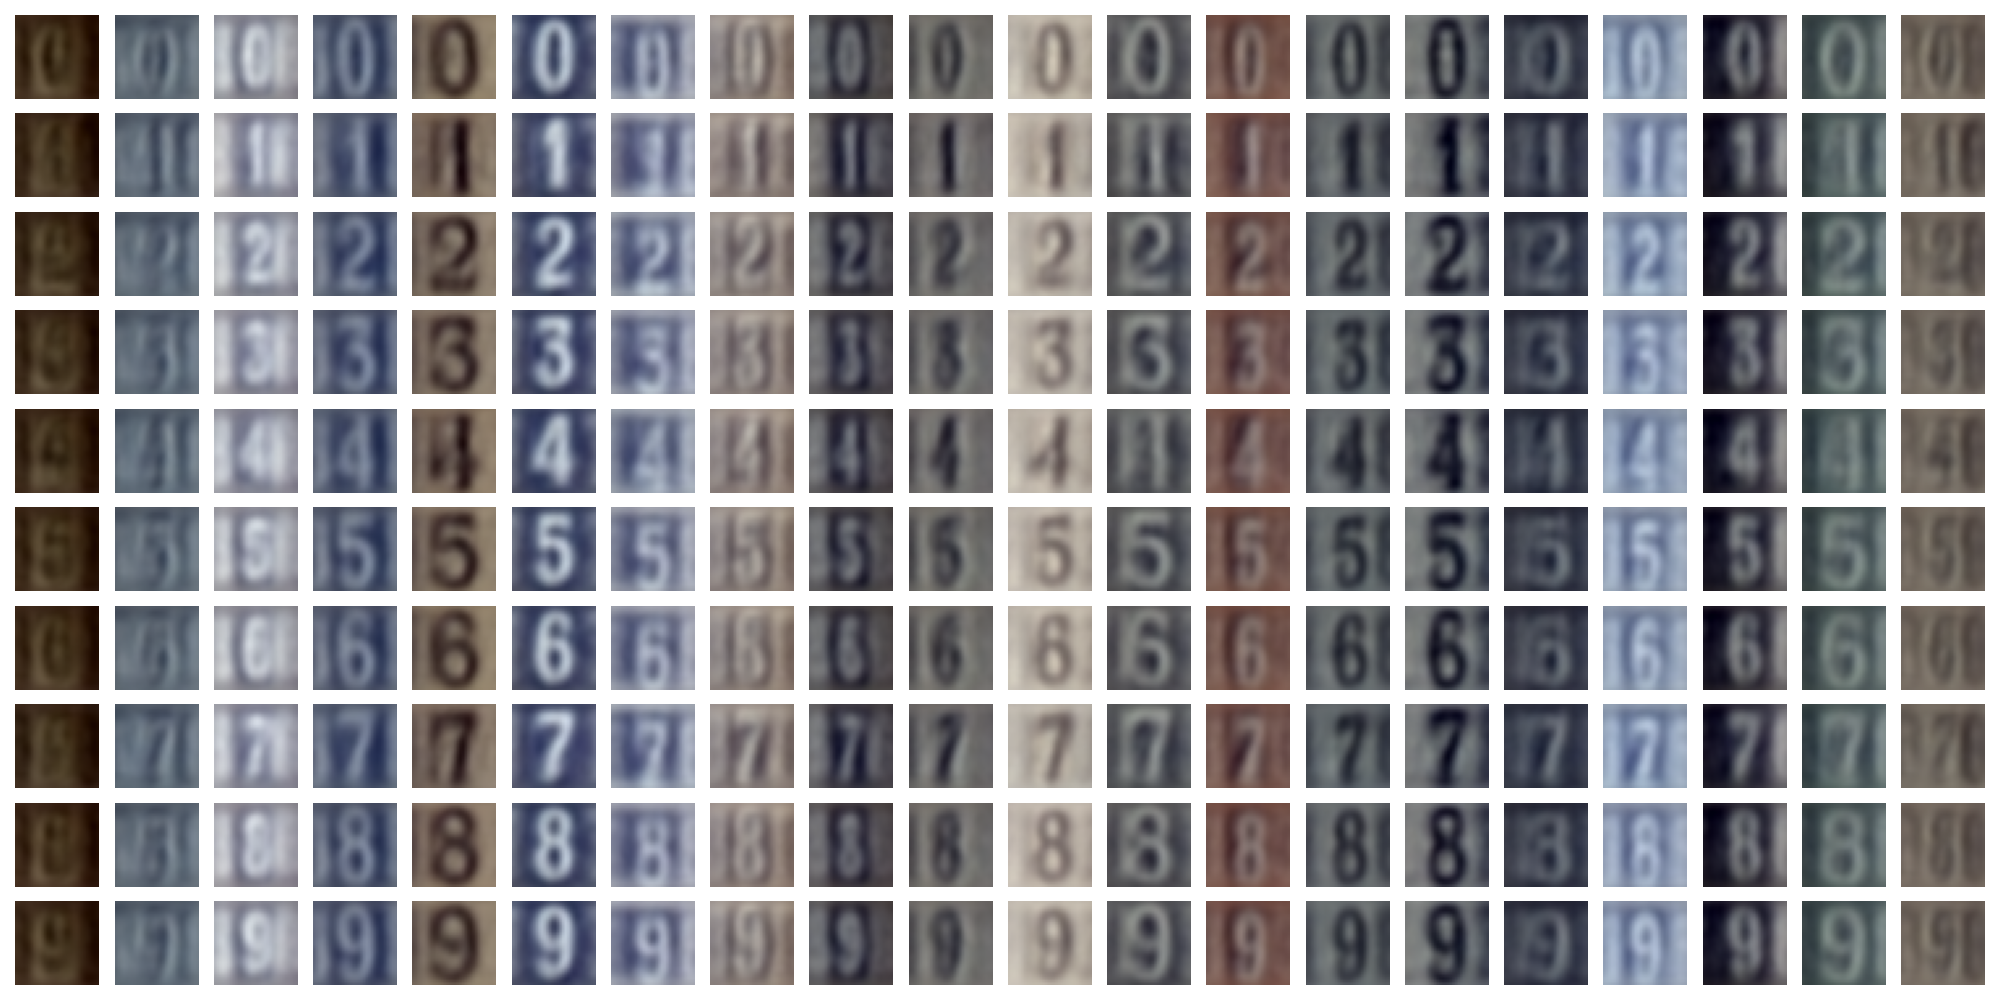
\includegraphics[width=0.4\textwidth]{./figures/fsvae_gen}
    \end{figure}

\end{enumerate}